\documentclass[12pt,letterpaper]{memoir}

\usepackage{xparse}
\usepackage{blindtext}
\usepackage{enumitem}
\usepackage{graphicx}

\usepackage{amsmath,mathtools,amssymb}
% See https://texblog.net/latex-archive/maths/amsmath-matrix/ 
% for an explanation of this extention of the amsmath matrix commands.
% It's a way to enable "augmented matrices" using a new optional argument:
%
% \begin{pmatrix}[cc|c]
%     1 & 2 & 3\\
%     4 & 5 & 9
%   \end{pmatrix}
%
\makeatletter
\renewcommand*\env@matrix[1][*\c@MaxMatrixCols c]{%
  \hskip -\arraycolsep
  \let\@ifnextchar\new@ifnextchar
  \array{#1}}
\makeatother

\usepackage{bm} % bold math package

\usepackage{booktabs}
\usepackage{multirow}
\usepackage{hyperref}
\usepackage{systeme}

\usepackage{tcolorbox}
    \tcbuselibrary{skins}
    \tcbuselibrary{raster}
    \tcbuselibrary{skins}
\usepackage{tikz}
    \usetikzlibrary{arrows.meta}
\usepackage{tkz-base}
\usepackage{tkz-fct}    
\usepackage{pgfplots}
    \pgfplotsset{compat=newest}

% for inserting blanks that the students fill in
\usepackage{dashundergaps} % for \gap
\dashundergapssetup{
    teacher-mode=false, % set to true to show answers 
    gap-format=underline,
    teacher-gap-format=underline,
    gap-font={\ECFAugie\MTversion{augie}\color{black}},
    gap-numbers=false,
    gap-widen=true,
    gap-extend-percent=100, % note: making this too big might create errors
    gap-number-format=\,\textsuperscript{\normalfont(\thegapnumber)},
}

\usepackage{emerald}
\usepackage[subdued]{mathastext}% no italic for Augie anyhow
    \MTDeclareVersion[n]{lmvtt}{T1}{lmvtt}{m}{n}
    \MTfamily{augie}
    \Mathastext[augie]

\newcommand{\myEmph}{\bfseries\itshape}
\newcommand{\myClassName}{{\tagged{pre-AP}{pre-AP }}Algebra 2}

% So I can save/restore \fboxsep
\newlength{\mySavedFboxsep}
\newcommand{\mySaveFboxsep}{\setlength{\mySavedFboxsep}{\fboxsep}}
\newcommand{\mySaveAndSetFboxsep}[1]{
    \setlength{\mySavedFboxsep}{\fboxsep}
    \setlength{\fboxsep}{#1}
}
\newcommand{\myRestoreFboxsep}{\setlength{\fboxsep}{\mySavedFboxsep}}

% A centered tcolorbox
%
% #1 - options to pass to tcolorbox
%
\NewDocumentEnvironment{myCenteredBox}{m}{%
    \begin{center}
    \begin{tcolorbox}[#1]
}{
    \end{tcolorbox}
    \end{center}
}


% A centered system of equations
%
\NewDocumentCommand{\myCenteredSysteme}{m}{%
    \begin{center}\systeme{#1}\end{center}
}

%
% This specialized command is my way of typesetting a table for
% students to use when solving systems of equations using matrices.
%
% - I make it really wide, because I need horizontal space. The increase in margin width 
%   is adjustable, but frankly, there are a lot of hard-coded dimensions in the table, so
%   I'm not positive that generality works well.
%
% - I put the content in a tikz picture with an OPAQUE background, since I 
%   plan to overlay this on top of Examples, which have dotted boxes around 
%   them at the "normal" margins.
%
% - The table uses the multirow package so that I can have the "Solution" box span two cells.
%
\NewDocumentCommand{\myWideMatrixTable}{O{-0.7in}}{
    \begin{adjustwidth}{#1}{#1}
        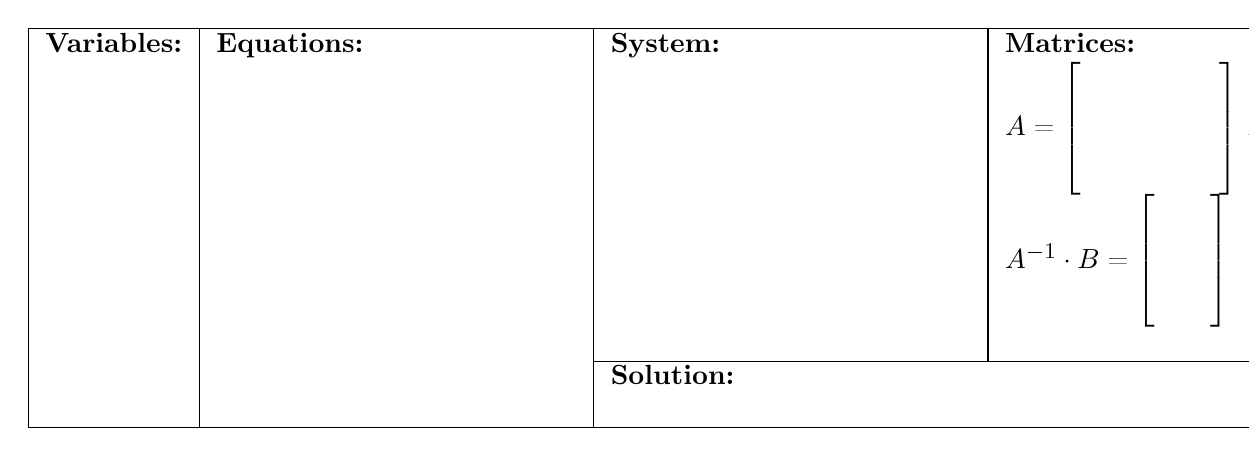
\begin{tikzpicture}
            \node
            [
                text width=1.25\textwidth, %I dinked with the multiplier to get balanced margins
                fill=white!30, 
                fill opacity=1,
                text opacity=1,
                inner sep=0pt,
            ]
            {%
                \begin{tabular}{|l|m{1.8in}|m{1.8in}|m{2.1in}|}
                    \hline
                    {\bfseries\scshape Variables:} & {\bfseries\scshape Equations:} & {\bfseries\scshape System:} & {\bfseries\scshape Matrices:} \\
                    % & & & \\
                    & & & 
                    \(
                        A = 
                        \begin{bmatrix}
                            \phantom{99} & \phantom{99} & \phantom{99} \\
                            \phantom{99} & \phantom{99} & \phantom{99} \\
                            \phantom{99} & \phantom{99} & \phantom{99} \\
                            \phantom{99} & \phantom{99} & \phantom{99} \\
                        \end{bmatrix}
                    \)
                    \(
                        B = 
                        \begin{bmatrix}
                            \phantom{999}\\
                            \phantom{999}\\
                            \phantom{999}\\
                            \phantom{999}\\
                    \end{bmatrix}
                    \)
                    \\
                    & & &
                    \(
                        A^{-1}\cdot B = 
                        \begin{bmatrix}
                            \phantom{9999}\\
                            \phantom{999}\\
                            \phantom{999}\\
                            \phantom{999}\\
                    \end{bmatrix}
                    \)
                    \\
                    & & & \\ \cline{3-4}
                    & & 
                    \multicolumn{2}{l|}{\bfseries\scshape Solution:}
                    \\ 
                    & & 
                    \multicolumn{2}{l|}{\,}
                    \\ 
                    \hline
                \end{tabular}
            };
        \end{tikzpicture}
    \end{adjustwidth}
}

% ---------------------------------------------------------------------------
% number lines using Tkz
% ---------------------------------------------------------------------------

% a simple number line
%
% #1 scale of the numberline
% #2 max x
% #3 min x (optional, if absent it defaults to negative of the max)
% #4 label on the x-axis (optional, if absent there's no label)
%
\NewDocumentCommand{\myNumberLine}{ O{0.4} m o O{{}} }{
    \begin{tikzpicture}[
        scale=#1,
        xaxe style/.style = { very thick, arrows={-{Straight Barb}}, },                 
        ]
        \tkzInit[ xmax=#2, xmin=\IfValueTF{#3}{#3}{-#2}, xstep=1, ]
        \tkzDrawX[
            % right=12pt,
            label=#4,
            noticks=false, % Yes, I want ticks!
            tickup=1em, tickdn=1em,
            right space=0.05cm, left space=0.05cm, % extend the line beyond the last ticks
            ]
        % \tkzLabelX[ 
        %     % orig=false,
        %     step=#4,
        %     font=\small,
        %     below left=2pt,
        %  ]
    \end{tikzpicture}
}


% ---------------------------------------------------------------------------
% x-y graphs using Tkz
% ---------------------------------------------------------------------------

% a tikzpicture wrapper environment that uses Tkz to draw an x-y grid
%
% #1 tikzpicture scale
%
% #2 optional xmin (defaults to negative of xmax)
% #3 xmax
% #4 optional ymin (defaults to negative of ymax)
% #5 ymax
%
\NewDocumentEnvironment{myTikzpictureGrid}{ m omom }{
    \begin{tikzpicture}[
        scale=#1,
        xaxe style/.style = { dashed, very thick, arrows={-{Straight Barb}}, },                 
        yaxe style/.style = { dashed, very thick, arrows={-{Straight Barb}}, },                 
        ]
        \tkzInit[
            xmin={\IfValueTF{#2}{#2}{-#3}}, xmax=#3, xstep=1,
            ymin={\IfValueTF{#4}{#4}{-#5}}, ymax=#5, ystep=1,
            ]
        \tkzGrid[ sub, subxstep=1, subystep=1, ]
        \tkzDrawX[label={$x$},color=black, right=0.2em,]
        \tkzDrawY[label={$y$},color=black, above=0.2em,]
        % \tkzLabelX[orig=false,] \tkzLabelY[orig=false,]
}{
    \end{tikzpicture}
}

% A counter to number the problems in the guided notes.
\newcounter{MyProblemCounter}
\setcounter{MyProblemCounter}{1}
\newcommand{\useMyProblemCounter}{\theMyProblemCounter\stepcounter{MyProblemCounter}}


% the style to use to render the problem counter on paper
\newcommand{\myProblemFont}{\bfseries\itshape}



% ---------------------------------------------------------------------------
% These are the commands I use to format the problems in the guided notes
% that have an empty space where I will write during class.
% ---------------------------------------------------------------------------

% A single problem that takes half the page.
%
% #1 : optional directions for the problem(s)
% #2 : details for problem 1
% #3 : optional font style for box titles
% #4 : vertical height of the problem boxes
% #5 : optional text at the bottom
%
\NewDocumentCommand{\myProblem}{ o m O{\normalsize} m O{} }{%
    \IfValueT{#1}{\vspace{1\parskip}\noindent#1\nopagebreak}%
    \begin{tcbraster}[%
        raster equal height,%
        raster columns=2,%
        raster column skip=0.5mm,%
        raster row skip=0.5mm,%
        ]%
        % This is the first problem.
        \begin{tcolorbox}[%
            enhanced,%
            sharp corners,%
            colback=white,%
            coltitle=black, colbacktitle=black!10!white,%
            boxrule=0pt, borderline={0.5pt}{0pt}{black},%
            title={\texttt{\useMyProblemCounter}},%
            attach boxed title to top left={xshift=-3mm,yshift=-3mm},%
            boxed title style = {size=small, drop fuzzy shadow southwest,},
            ]
            #3#2
            \tcblower\vspace{#4}#5
        \end{tcolorbox}
        %
        % There IS no second problem. So make it empty space.
        \begin{tcolorbox}[colback=white, colframe=white,]\end{tcolorbox}%
    \end{tcbraster}
}

% A single problem that takes the full width of the page.
%
% #1 : optional directions for the problem(s)
% #2 : details for problem 1
% #3 : optional font style for box titles
% #4 : vertical height of the problem boxes
% #5 : optional text at the bottom
%
\NewDocumentCommand{\myWideProblem}{ o m O{\normalsize} m O{} }{%
    \IfValueT{#1}{\vspace{1\parskip}\noindent#1\nopagebreak}%
    \begin{tcbraster}[%
        raster equal height,%
        raster columns=1,%
        raster column skip=0.5mm,%
        raster row skip=0.5mm,%
        ]%
        % This is the first problem.
        \begin{tcolorbox}[%
            enhanced,%
            sharp corners,%
            colback=white,%
            coltitle=black, colbacktitle=black!10!white,%
            boxrule=0pt, borderline={0.5pt}{0pt}{black},%
            title={\texttt{\useMyProblemCounter}},%
            attach boxed title to top left={xshift=-3mm,yshift=-3mm},%
            boxed title style = {size=small, drop fuzzy shadow southwest,},
            ]
            #3#2
            \tcblower\vspace{#4}#5
        \end{tcolorbox}
    \end{tcbraster}
}

% Two problems next to each other.
%
% #1 : optional directions for the problem(s)
% #2 : details for problem 1
% #3 : details for problem 2
% #4 : optional font style for box titles
% #5 : vertical height of the problem boxes
% #6 : optional text at the bottom of problem 1
% #7 : optional text at the bottom of problem 2
%
\NewDocumentCommand{\myProblems}{ o m m O{\normalsize} m O{} O{#6} }{%
    \IfValueT{#1}{\vspace{1\parskip}\noindent#1\nopagebreak}%
    \begin{tcbraster}[%
        raster equal height,%
        raster columns=2,%
        raster column skip=0.5mm,%
        raster row skip=0.5mm,%
        ]%
        % This is the first problem.
        \begin{tcolorbox}[%
            enhanced,%
            sharp corners,%
            colback=white,%
            coltitle=black, colbacktitle=black!10!white,%
            boxrule=0pt, borderline={0.5pt}{0pt}{black},%
            fonttitle=\small,
            title={\texttt{\useMyProblemCounter}},%
            attach boxed title to top left={xshift=-3mm,yshift=-3mm},%
            boxed title style = {size=small, drop fuzzy shadow southwest,},
            ]
            #4#2
            \tcblower\vspace{#5}#6
        \end{tcolorbox}
        % This is the second problem. 
        \begin{tcolorbox}[%
            enhanced,%
            sharp corners,%
            colback=white,%
            coltitle=black, colbacktitle=black!10!white,%
            boxrule=0pt, borderline={0.5pt}{0pt}{black},%
            fonttitle=\small,
            title={\texttt{\useMyProblemCounter}},%
            attach boxed title to top right={xshift=3mm,yshift=-3mm},%
            boxed title style = {size=small, drop fuzzy shadow southeast,},
            ]
            #4#3
            \tcblower\vspace{#5}#7
        \end{tcolorbox}
    \end{tcbraster}
}

% ---------------------------------------------------------------------------
% These are the commands I use to format the problems in the guided notes
% that have an partially filled space where I will also write during class.
%
% I use the term "with content" to refer to this partially filled space.
% ---------------------------------------------------------------------------

% A single problem that takes half the page.
%
% #1 : optional directions
% #2 : the problem contents
% #3 : optional font style for the content
%
\NewDocumentCommand{\myProblemWithContent}{ o m O{\normalsize} }{%
    \IfValueT{#1}{\vspace{1\parskip}\noindent#1\nopagebreak}%
    \begin{tcbraster}[%
        raster equal height,%
        raster columns=2,%
        raster column skip=0.5mm,%
        raster row skip=0.5mm,%
        ]%
        % This is the first problem.
        \begin{tcolorbox}[%
            enhanced,%
            sharp corners,%
            colback=white,%
            coltitle=black, colbacktitle=black!10!white,%
            boxrule=0pt, borderline={0.5pt}{0pt}{black},%
            title={\texttt{\useMyProblemCounter}},%
            attach boxed title to top left={xshift=-3mm,yshift=-3mm},%
            boxed title style = {size=small, drop fuzzy shadow southwest,},
            ]
            #3#2
        \end{tcolorbox}
        %
        % There IS no second problem. So make it empty space.
        \begin{tcolorbox}[colback=white, colframe=white,]\end{tcolorbox}%
    \end{tcbraster}
}


% Two problems that that sit next to each other.
%
% #1 : optional directions
% #2 : the 1st problem contents
% #3 : the 2nd problem contents
% #4 : optional font style for the content
%
\NewDocumentCommand{\myProblemsWithContent}{ o m m O{\normalsize} }{%
    \IfValueT{#1}{\vspace{1\parskip}\noindent#1\nopagebreak}%
    \begin{tcbraster}[%
        raster equal height,%
        raster columns=2,%
        raster column skip=0.5mm,%
        raster row skip=0.5mm,%
        ]%
        % This is the first problem.
        \begin{tcolorbox}[%
            enhanced,%
            sharp corners,%
            colback=white,%
            coltitle=black, colbacktitle=black!10!white,%
            boxrule=0pt, borderline={0.5pt}{0pt}{black},%
            title={\texttt{\useMyProblemCounter}},%
            attach boxed title to top left={xshift=-3mm,yshift=-3mm},%
            boxed title style = {size=small, drop fuzzy shadow southwest,},
            ]
            #4#2
        \end{tcolorbox}
        % This is the second problem.
        \begin{tcolorbox}[%
            enhanced,%
            sharp corners,%
            colback=white,%
            coltitle=black, colbacktitle=black!10!white,%
            boxrule=0pt, borderline={0.5pt}{0pt}{black},%
            title={\texttt{\useMyProblemCounter}},%
            attach boxed title to top left={xshift=3mm,yshift=-3mm},%
            boxed title style = {size=small, drop fuzzy shadow southeast,},
            ]
            #4#3
        \end{tcolorbox}
    \end{tcbraster}
}


% A wide problem that can have any latex code in the content area of the box.
%
% #1 : optional directions 
% #2 : the problem
% #3 : optional font style for the content
%
\NewDocumentCommand{\myWideProblemWithContent}{ o m O{\normalsize} }{%
    \IfValueT{#1}{\vspace{1\parskip}\noindent#1\nopagebreak}%
    \begin{tcbraster}[%
        raster equal height,%
        raster columns=1,%
        raster column skip=0.5mm,%
        raster row skip=0.5mm,%
        ]  
        \begin{tcolorbox}[%
            enhanced,%
            sharp corners,%
            colback=white,%
            coltitle=black, colbacktitle=black!10!white,%
            boxrule=0pt, borderline={0.5pt}{0pt}{black},%
            title={\texttt{\useMyProblemCounter}},%
            attach boxed title to top left={xshift=-3mm,yshift=-3mm},%
            boxed title style = {size=small, drop fuzzy shadow southwest,},
            ]%
            #3#2
        \end{tcolorbox}
    \end{tcbraster}
}

\newenvironment{myVocabulary}{
    \begin{myTabularAnnotate}{Vocabulary}{}
}{
    \end{myTabularAnnotate}
}
\newcommand{\myDefinition}[2]{
    \myRow{#1}{#2}
}
\newcommand{\myCourse}{\whenHONORS{Honors~}Algebra 2}
\newcommand{\myAssignmentName}{\whenHONORS{H-}Review 4.3--4.4}


% A command to print the header at the top of an assignment.
%
% #1 course name
% #2 assignment name
%
\NewDocumentCommand{\myAssignmentHeader}{O{Algebra 2} O{Assignment}}{%
    \noindent
    #1
    \hfill 
    Name : \fbox{\phantom{\large Xxxxxx Xxxxxx-Xxxxxx}}

    \vspace{0.5em}

    \noindent
    {\Large\bfseries\sffamily#2}
    \hfill 
    Period : \fbox{\phantom{\large 9999}}

    \hrule\hspace{\baselineskip}
}



% memoir commands to define the text block geometry
\setulmarginsandblock{0.5in}{*}{*}
\setlrmarginsandblock{0.5in}{*}{*} % leave space in left margin for punched holes
% memoir command to enable subsection numbering
\setsecnumdepth{subsection}


% logic to reduce subscript size 
% See: https://tex.stackexchange.com/questions/262295/make-subscript-size-smaller-always 
%
\catcode`_=\active
\newcommand_[1]{\ensuremath{\sb{\scriptscriptstyle #1}}}


% the background color for student-fill-in tcolorboxes
\newcommand{\myFillinColor}{black!20}


\newcommand{\mymm}{{\bfseries\itshape m\&m}}
\setlength{\parindent}{0em}
\setlength{\parskip}{1ex}


\begin{document}
\pagestyle{plain}
\checkandfixthelayout
\raggedbottom

\forHONORS
\dashundergapssetup{
    teacher-mode=true, % set to true to show answers 
}
\myAssignmentHeader[\whenHONORS{Honors~}Algebra 2][\whenHONORS{H-}Catapult Project]

This is a {\bfseries\itshape three--day project} in which you will:
\begin{itemize}[nosep,]
    \item build a catapult, 
    \item launch \mymm{}s using the catapult,
    \item collect data about the \mymm~trajectories,
    \item explore parabolic models for the \mymm~trajectories.
\end{itemize}

\begin{myVocabulary}
    \myDefinition{catapult}{a machine that throws things in the air}
    \myDefinition{trajectory}{the path followed by something moving through space}
    \myDefinition{model}{a function that helps you predict things}
    \myDefinition{predict}{saying what you think will happen before it actually happens}
    \myDefinition{parabolic}{shaped like a parabola, like the graph of a quadratic function}
\end{myVocabulary}

\section{Getting Started (Day 1)}

\myCenteredBox[width=5in,colback=white,sharp corners,]{
    Today you will 
    \begin{itemize}[nosep,label=\checkmark]
        \item break into teams,
        \item build catapults,
        \item test them with \mymm{}s, and 
        \item practice taking measurements.
    \end{itemize}
}


\subsection{Teams}

You may work in groups of up to 4 people. Or you may work on your own.
There are four ``roles''. If you have several people on your team, 
each person must have a role. Record that information here.

\myCenteredBox[colback=\myFillinColor]{
    \centering
    \renewcommand{\arraystretch}{1.5}
    \begin{tabular}{l|p{3in}|p{3in}}
        \toprule
        {\itshape role} & {\itshape what?} & {\itshape who?} \\
        \toprule
        {\bfseries\itshape launcher} & hold and launch the catapult. & \\
        \midrule
        {\bfseries\itshape timer}    & time the flight of the \mymm{}s&\\
        \midrule
        {\bfseries\itshape measurer} & measure how far the \mymm~flew&\\
        \midrule
        {\bfseries\itshape recorder} & write down all the times and measurements&\\
        \bottomrule
    \end{tabular}
}

\subsection{Catapult Construction}

Each team will build a catapult from tongue depressor sticks and rubber bands.
Here are the steps.
Check them off when you have completed them.
\myCenteredBox[colback=\myFillinColor]{
    \begin{itemize}[label={\Large$\Box$}]
        \item Wind a rubber band several times around one end of a stick 
            so that the rubber band stays in place.
            Your \mymm{}s will rest against this rubber band when you launch.
        \item Put a second stick next to the first one. Wrap a rubber band around the other end of them
            to hold them tightly together. 
        \item Insert a pencil between the two sticks. 
            You might want to use more rubber bands so that the pencil 
            does not easily move back and forth.
            The gap created by the pencil is what makes the catapult ``spring''.
    \end{itemize}
}

If you do not understand these instructions, look at the catapults of other teams, or come look at mine.
If you do not understand how the catapult works, ask me to show you.

Give your catapult a {name}.
\myCenteredBox[colback=\myFillinColor]{
    \centering
    {\itshape name:} \fbox{\phantom{\LARGE Xxxxxx Xxxxxx-Xxxxxx}}
}

\subsection{Dry Runs}

Now it is time to try out your catapult. 
Find a clear space, and try launching an \mymm. 
This will give you a feel for how it works and how much space you need.

Here is the general idea.
\begin{itemize}[nosep]
    \item You will launch your \mymm{}s from your catapult.
    \item The candy will fly across the room following a parabolic trajectory.
    \item The candy will {\scshape Land} at a point ``downrange'' of the {\scshape Launch} point.
    \item You will measure the downrange distance.
    \item You will time how long the candy is in the air (from launch to landing).
\end{itemize}

\begin{center}
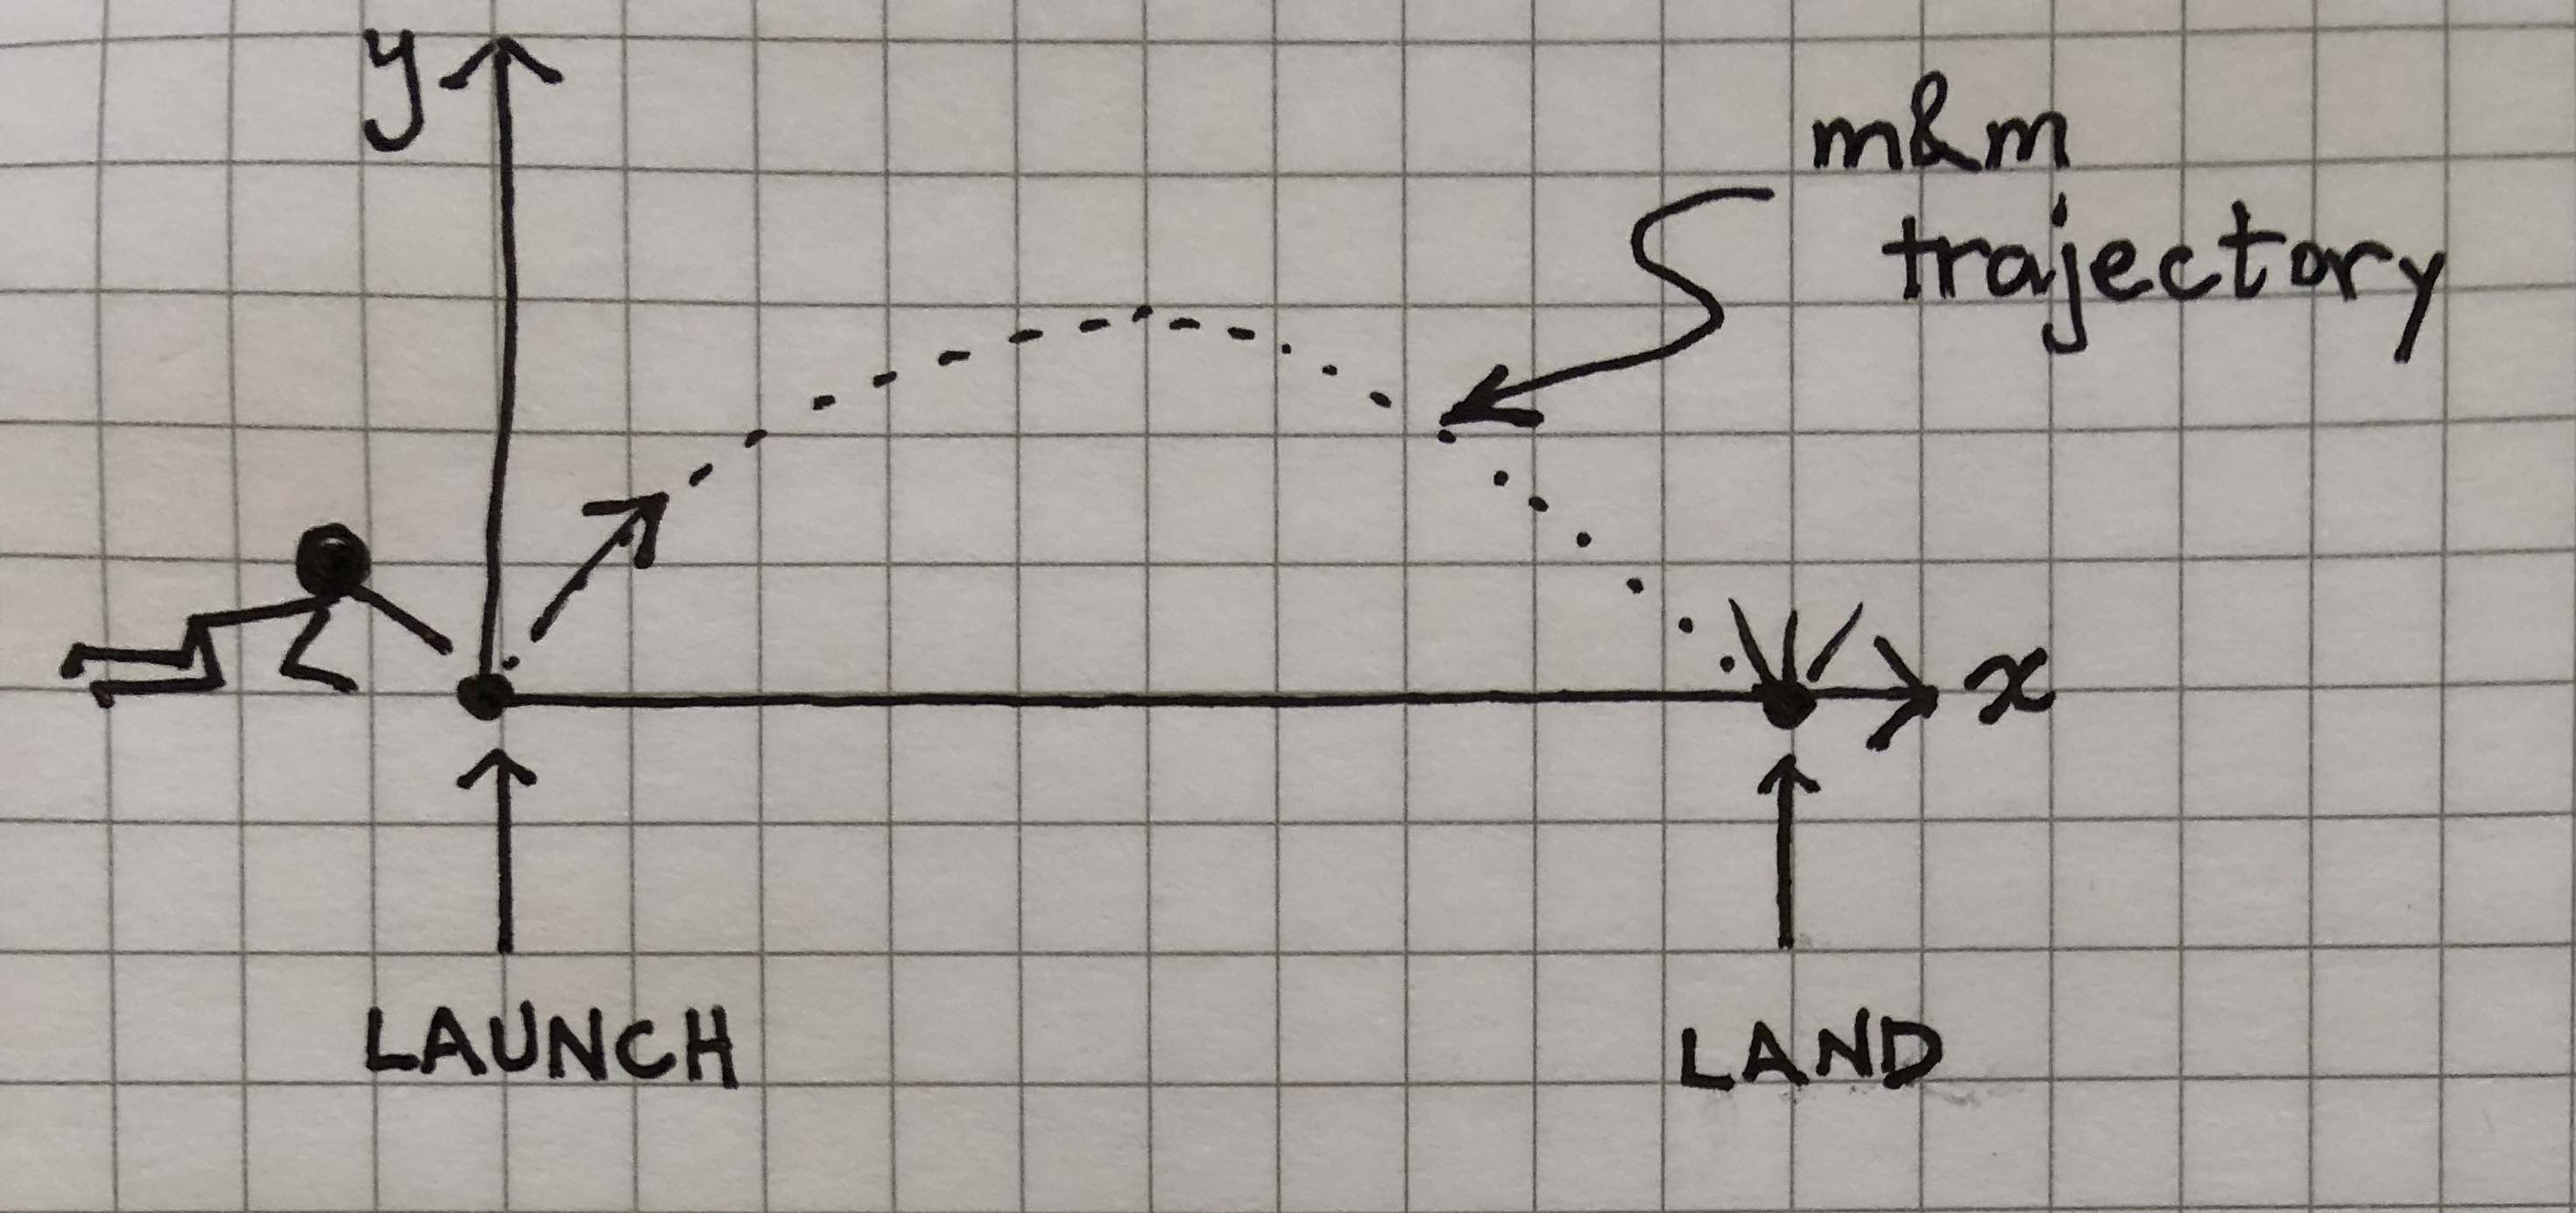
\includegraphics[width=3in]{../launch-and-landing.jpg}
\end{center}

Practice timing and measuring the flight of your \mymm{}s. 
Launch {\bfseries\itshape at least 3} \mymm{}s. 
\begin{itemize}[nosep]
    \item The {\bfseries\itshape timer} person should use their phone to determine 
        the {\bfseries\itshape flight time} (in seconds) of each test trajectory.
    \item The {\bfseries\itshape measurer} should use a yardstick to measure 
        the {\bfseries\itshape downrange distance} (in centimeters) of each test trajectory.
    \item The {\bfseries\itshape recorder} should write those values down.
    \item Everyone should copy those values into their packets below.
\end{itemize}

\myCenteredBox[colback=\myFillinColor]{
    \centering
    \renewcommand{\arraystretch}{1.5}
    \begin{tabular}{c|p{2in}|p{2in}}
        \toprule
        {\itshape dry run \#} & {\itshape fight time (sec)} & {\itshape downrange distance (cm)} \\
        \toprule
        1 & & \\
        \midrule
        2 & & \\
        \midrule
        3 & & \\
        \bottomrule
    \end{tabular}
}

Are your times and distances all approximately the same? 
\myCenteredBox[colback=\myFillinColor]{
    \centering 
    \qquad
    {\scshape Yes}
    \qquad
    {\scshape No}
    \qquad
    (circle one)
}

If not, write a short explanation of what was different and 
what you think explains the difference.%
\footnote{%
    For example:%
    ``The second dry run was messed up since we didn't 
    start timing right when the catapault launched.''
}

\myCenteredBox[colback=\myFillinColor]{
    \vspace{1em}
    \underline{\hspace{\textwidth}}\\[0.5\baselineskip]
    \underline{\hspace{\textwidth}}\\[0.5\baselineskip]
    \underline{\hspace{\textwidth}}\\[0.5\baselineskip]
    \underline{\hspace{\textwidth}}\\[0.5\baselineskip]
    \underline{\hspace{\textwidth}}\\[0.5\baselineskip]
    \underline{\hspace{\textwidth}}\\
}

\newpage 
\section{A Quadratic Trajectory Function (Day 2)}

\myCenteredBox[width=5in,colback=white,sharp corners,]{
    Today you will 
    \begin{itemize}[nosep,label=\checkmark]
        \item Launch \mymm{}s from your catapult.
        \item Time and measure the \mymm~trajectories.
        \item Find a quadratic model that describes the trajectories.
    \end{itemize}
}





\subsection{The General Idea}

The trajectories you tested yesterday are {\bfseries\itshape parabolic}---%
they can be modeled as a quadratic function:
\begin{equation}\label{parabolic-model}
    y = \bm{a}(x-\bm{h})^2 + \bm{k}
\end{equation} 
where 
\begin{itemize}[nosep]
    \item $y$ is the vertical height of the \mymm~trajectory, 
    \item $x$ is the horizontal distance of the \mymm{}s from the catapult, and
\end{itemize}

Today 
{\bfseries\itshape you will find} the values of $\bm{a}$, $\bm{h}$, $\bm{k}$.
Once you find the them, 
you may substitute them into Equation (\ref{parabolic-model}) to get a 
quadratic model of your \mymm~trajectories.





\subsection{DAY 2 Geometry}

There are three points on the parabolic trajectory that are important.
\begin{itemize}[nosep]
    \item $\bm{A}$, the launch point (the $x$-intercept where the catapult is),
    \item $\bm{V}$, the highest point (vertex) of the trajectory, and
    \item $\bm{B}$, the landing point (the $x$-intercept where the \mymm{}s land). 
\end{itemize}

\begin{center}
    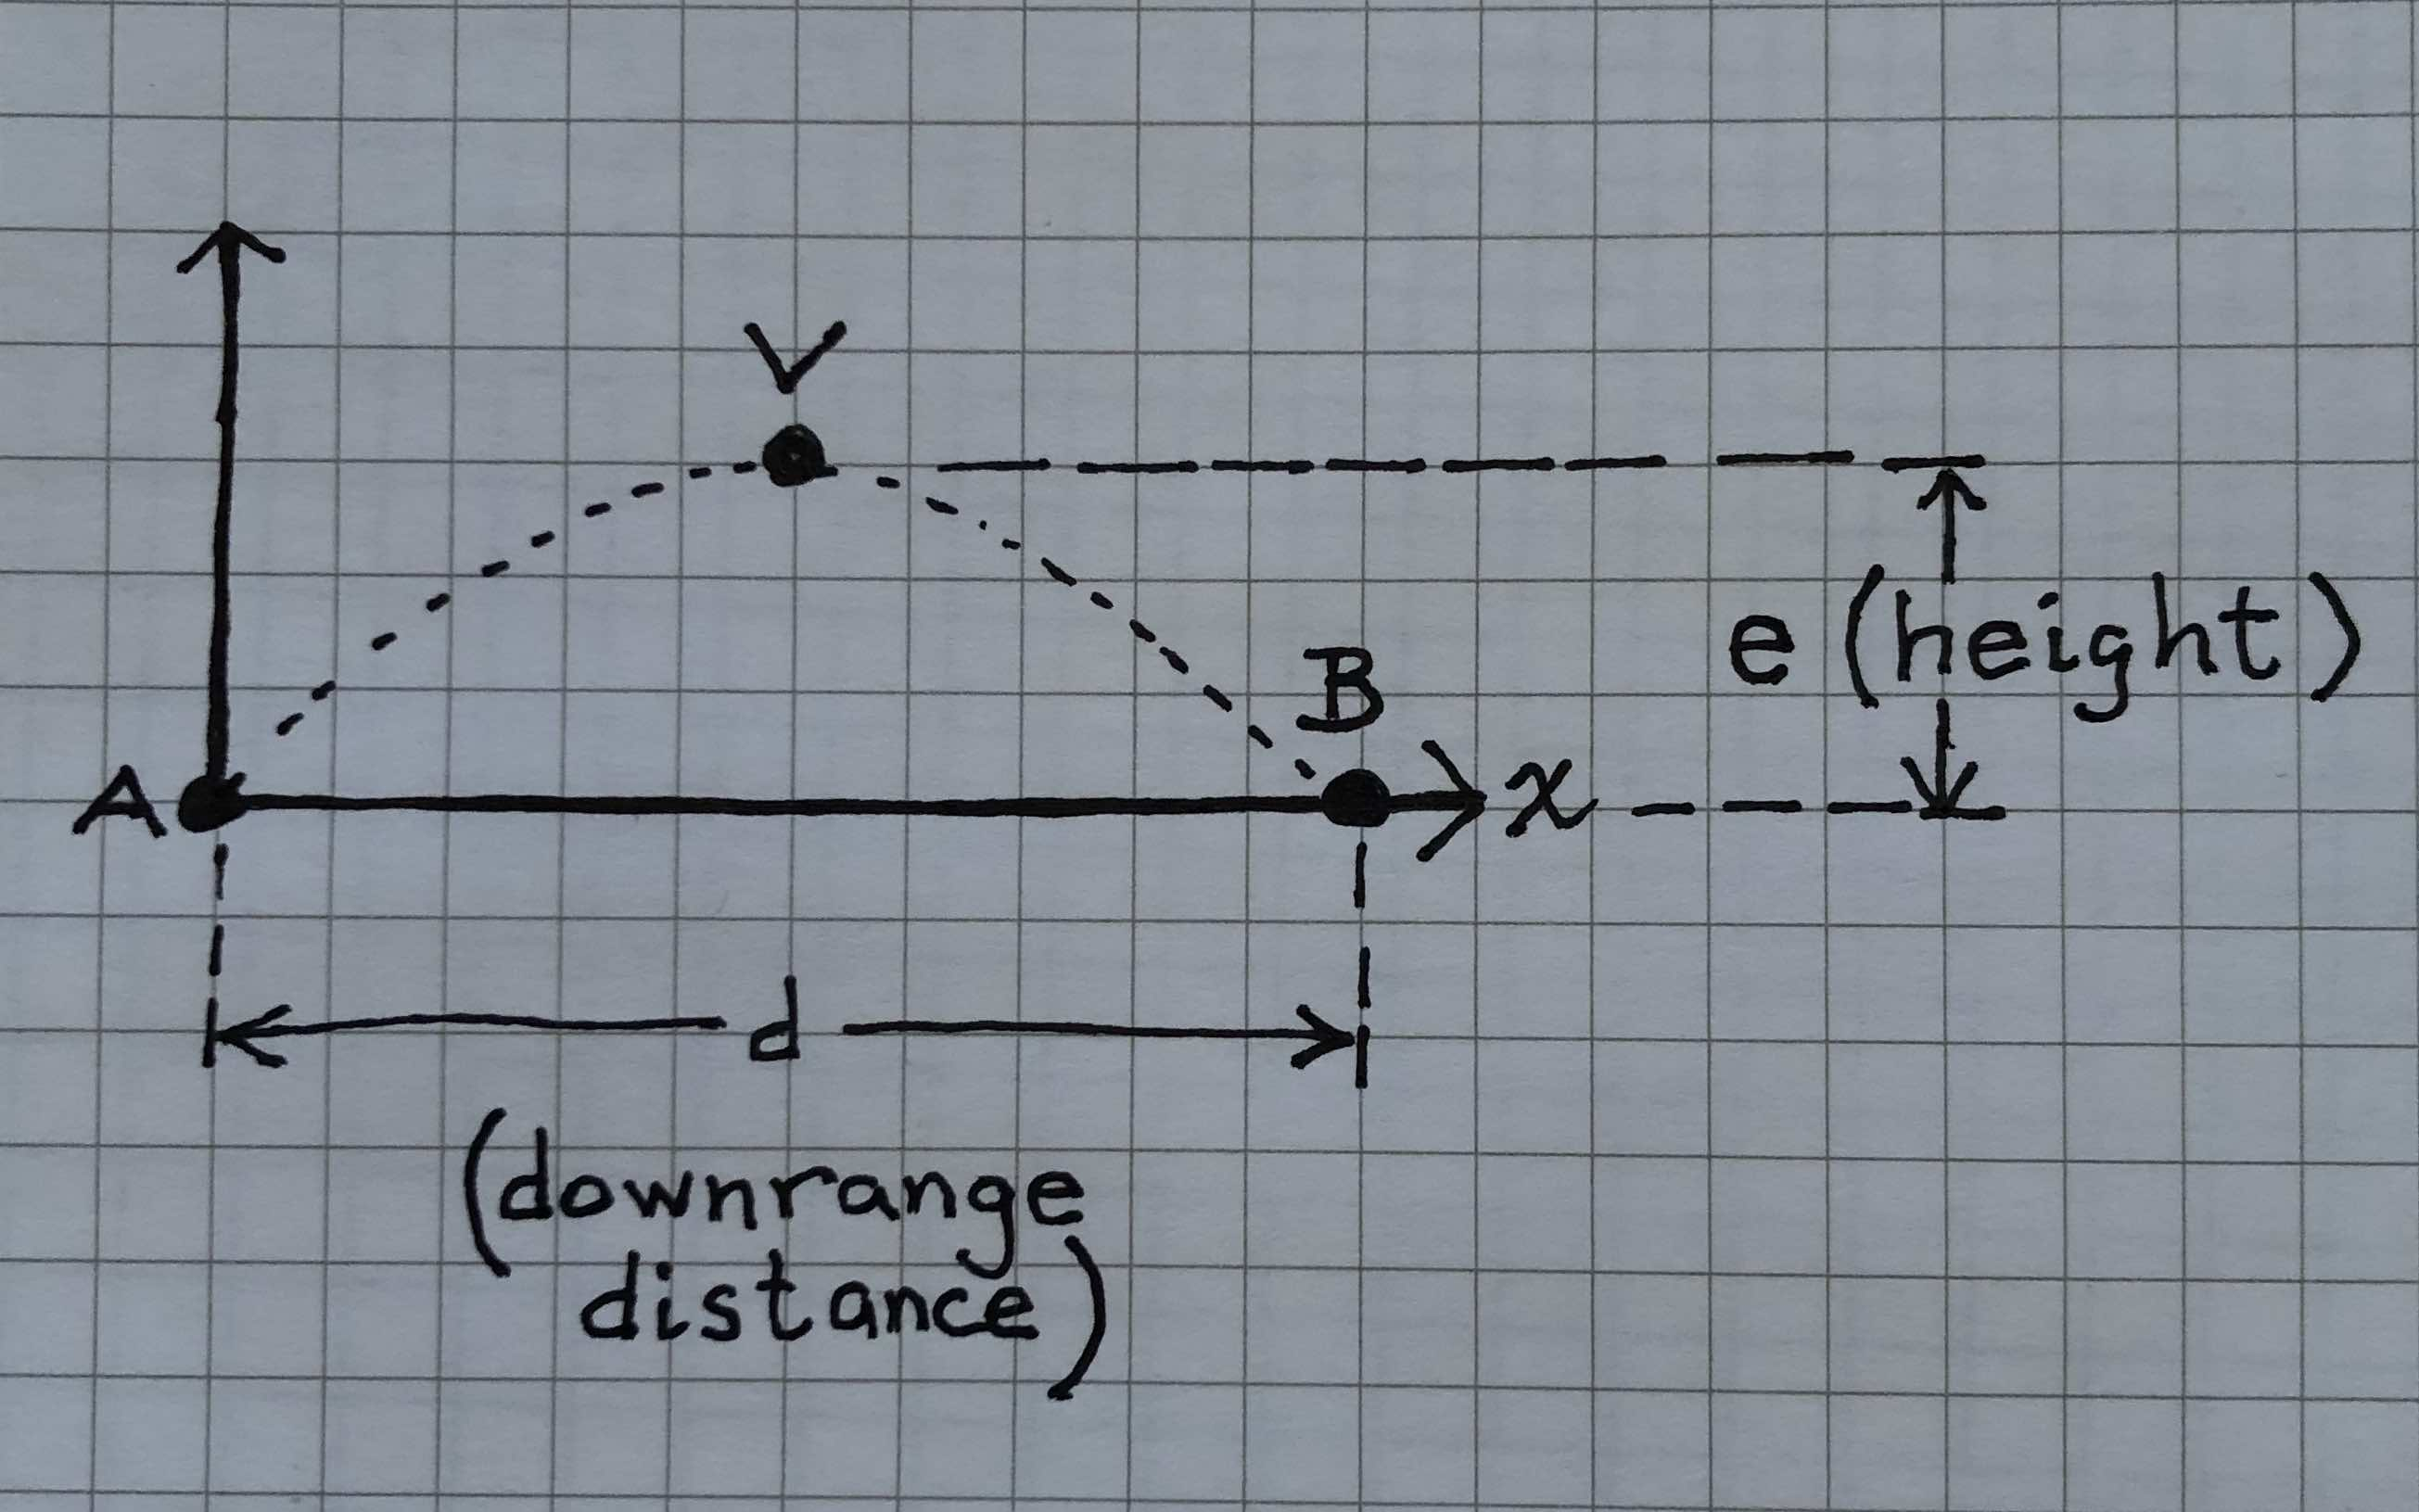
\includegraphics[width=3in]{../AVB.jpg}
\end{center}

You can find the $(x, y)$ coordinates of each of these points, 
once you calculate $d$ and $e$.





\subsection{Launch Data Collection}

Launch your catapult three times.
For each launch,
\begin{itemize}[nosep]
    \item Your group's {\bfseries\itshape timer} person should 
        measure the {\itshape flight time} in seconds using a phone timer.
    \item Your group's {\bfseries\itshape measuring} person should 
        measure {\itshape downrange distance} 
        in centimeters using a yardstick.
    \item Your group's {\bfseries\itshape recording} person should 
        write down the flight time and downrange distance.
\end{itemize}
\myCenteredBox[colback=\myFillinColor]{
    \centering
    \renewcommand{\arraystretch}{1.5}
    \begin{tabular}{c|p{2in}|p{2in}}
        \toprule
        {\itshape launch \#} & {\itshape flight time (sec)} & {\itshape downrange distance (cm)} \\
        \toprule
        1 & & \\
        \midrule
        2 & & \\
        \midrule
        3 & & \\
        \bottomrule
    \end{tabular}
}

Average your measurements.

\begin{tcolorbox}[colback=\myFillinColor,ams align]
    \text{\itshape average downrange distance} = 
    ( 
        \text{\gap{???}} +  \text{\gap{???}} + \text{\gap{???}}
    ) / 3 
    = \text{\gap{???}}
\end{tcolorbox}
\begin{tcolorbox}[colback=\myFillinColor,ams align]
    \text{\itshape average flight time} 
    = 
    ( \text{\gap{???}} +  \text{\gap{???}} + \text{\gap{???}}) / 3 
    = \text{\gap{???}}
\end{tcolorbox}
    


\subsection{Finding $d$ and $e$}

$d$ is the average downrange distance.
\begin{tcolorbox}[colback=\myFillinColor,ams align]
    d 
    = \text{\itshape average downrange distance} 
    = \text{\gap{???}}
\end{tcolorbox}

The time to reach the highest point is one-half the average flight time,
since it occurs in the middle.
\begin{tcolorbox}[colback=\myFillinColor,ams align]
    t_{peak} 
    = \frac{1}{2} (\text{\itshape average flight time})
    = \text{\gap{???}}
\end{tcolorbox}

$e$ comes from phyics: $e = \frac{1}{2}gt^2$, 
where 
$g = 980~cm/s^2$.
\begin{tcolorbox}[colback=\myFillinColor,ams align]
    e & = \frac{1}{2} \cdot g \cdot t^2_{peak} \\
      & = \frac{1}{2} \cdot 980 \cdot (\text{\gap{?????}})^2\\
      & = \text{\gap{?????}}
\end{tcolorbox}





\subsection{The Coordinates of $\bm{A}$, $\bm{V}$, and $\bm{B}$}

The launch point is at the origin.
You know its coordinates.
So $\bm{A}$'s coordinates are
\begin{tcolorbox}[colback=\myFillinColor,ams align]\label{A-coords}
    (x, y)^{}_{\bm{A}} = ( \text{\gap{0}}, \text{\gap{0}})
\end{tcolorbox}
    
The landing point $\bm{B}$ is an $x$-intercept located 
a horizontal distance $d$ from the origin.
But you just found $d$.
So $\bm{B}$'s coordinates are
\begin{tcolorbox}[colback=\myFillinColor,ams align]
    (x, y)^{}_{\bm{B}} = ( \text{\gap{d}}, \text{\gap{0}})
\end{tcolorbox}

The point $\bm{V}$ is located
\begin{itemize}[nosep]
    \item horizontally halfway from $\bm{A}$ to $\bm{B}$,
        which is $\frac{1}{2}d$, and
    \item vertically $e$ units above the $x$-axis.
\end{itemize}
You found $d$ and $e$ above, so $\bm{V}$'s coordinates are 
\begin{tcolorbox}[colback=\myFillinColor,ams align]
    (x, y)^{}_{\bm{V}} &= ( d/2, e)\\ \label{vertex-coords}
    (x, y)^{}_{\bm{V}} &= ( \text{\gap{d/2}}, \text{\gap{e}})
\end{tcolorbox}





\subsection{The Quadratic Trajectory Model}

The quadratic function that models your trajectory 
was mentioned in Equation \ref{parabolic-model} on page~\pageref{parabolic-model}.
We need to find the values of $\bm{a}$, $\bm{h}$, and $\bm{k}$.

The point $\bm{V}$ is the {\bfseries\itshape vertex} with coordinates $(h, k)$.
But you already calculated the coordinates of $\bm{V}$!
(See Equation~\ref{vertex-coords}.)
So $h$ is the $x$-coordinate
and $k$ is the $y$-coordinate 
of $\bm{V}$:
%
\begin{tcolorbox}[colback=\myFillinColor,ams align]\label{h-value}
    h &= \text{\gap{???}}\\
    \label{k-value}
    k &= \text{\gap{???}}
\end{tcolorbox}
%
which means that the quadratic trajectory model (so far) is 
%
\begin{tcolorbox}[colback=\myFillinColor,ams align]\label{model-with-hk}
    y = \bm{a}(x-\text{\gap{h}})^2 + \text{\gap{k}}
\end{tcolorbox}
%
To find the value of $\bm{a}$, 
substitute the coordinates of either $\bm{A}$ or $\bm{B}$  
into this equation.
That will give you and equation that you can solve for $a$.

\myCenteredBox[colback=white,width=3in]{
    Hint: The coordinates of $\bm{A}$ are easiest.
    So use them!
}

The values of $x$ and $y$ at the point $\bm{A}$ 
from Equation~\ref{A-coords} 
are 
\begin{tcolorbox}[colback=\myFillinColor,ams align]
    x_{\bm{A}} &= \text{\gap{0}} \label{xa}\\
    y_{\bm{A}} &= \text{\gap{0}} \label{ya}
\end{tcolorbox}
%
Substitute those two values into Equation~\ref{model-with-hk}.
\begin{tcolorbox}[colback=\myFillinColor,ams align]
    y_{\bm{A}}     &= \bm{a}(x_{\bm{A}}-\text{\gap{h}})^2 + \text{\gap{k}} \label{solve-this-for-a}\\
    \text{\gap{0}} &= \bm{a}(\text{\gap{0}}-\text{\gap{h}})^2 + \text{\gap{k}} \\
    \text{\gap{0}} &= \bm{a}(-\text{\gap{h}})^2 + \text{\gap{k}} \\
    \text{\gap{0}} &= \bm{a} \cdot \text{\gap{???}} + \text{\gap{k}} 
\end{tcolorbox}
%
You can easily solve this for $\bm{a}$. 
Show your work here.
\begin{tcolorbox}[colback=\myFillinColor]
    \vspace{1in}
\end{tcolorbox}
And write your solution here.
\begin{tcolorbox}[colback=\myFillinColor,ams align]\label{a-value}
    \bm{a} = \text{\gap{???}}
\end{tcolorbox}

Your quadratic trajectory model is Equation~\ref{parabolic-model}.
\begin{equation*}
y = \bm{a}(x-\bm{h})^2 + \bm{k}
\end{equation*}

Substituting your values of $\bm{a}$ in Equation~\ref{a-value} 
and $\bm{h}$ and $\bm{k}$ in 
Equation~\ref{model-with-hk},
gives you your quadratic model 
for the catapult trajectories:
%
\begin{tcolorbox}[colback=\myFillinColor,ams align]\label{model-with-ahk}
    y = \text{\gap{a}}(x-\text{\gap{h}})^2 + \text{\gap{k}}
\end{tcolorbox}




\whenHONORS{
\subsection{What About Point $\bm{B}$?}

When you solved Equation~(\ref{solve-this-for-a}) for $\bm{a}$ above, 
you substituted the coordinates of the launch point $\bm{A}$.
Redo the calculation using the coordinates of landing point $\bm{B}$ instead. 
Is this solution for $\bm{a}$ the same as the one above?
\myCenteredBox[colback=\myFillinColor]{
    \centering 
    \qquad
    {\scshape Yes}
    \qquad
    {\scshape No}
    \qquad
    (circle one)
}

Explain why you think this does (or does not) make sense.

\myCenteredBox[colback=\myFillinColor]{
    \vspace{1em}
    \underline{\hspace{\textwidth}}\\[0.5\baselineskip]
    \underline{\hspace{\textwidth}}\\[0.5\baselineskip]
    \underline{\hspace{\textwidth}}\\[0.5\baselineskip]
    \underline{\hspace{\textwidth}}\\[0.5\baselineskip]
    \underline{\hspace{\textwidth}}\\[0.5\baselineskip]
    \underline{\hspace{\textwidth}}\\[0.5\baselineskip]
    \underline{\hspace{\textwidth}}\\[0.5\baselineskip]
    \underline{\hspace{\textwidth}}\\
}
}
\section{A Vertical Translation Upward (Day 3)}

\myCenteredBox[width=5.5in,colback=white,sharp corners,]{
    Today you will 
    \begin{itemize}[nosep,label=\checkmark]
        \item Transform yesterday's quadratic model using a vertical shift.
        \item Predict what happens if you launch \mymm{}s from a higher place.
        \item Test your prediction.
    \end{itemize}
}


\end{document}